\documentclass{article}
\usepackage{graphicx}
\usepackage{siunitx}
\graphicspath{ {images/} }
\title{Cannon Maximum Range}
\author{Grant Curell}
\begin{document}
\maketitle{}
\section{Problem}
and it shoots 10-kilogram cannonballs.
\\\\
Holzner, Steven. Physics I For Dummies (For Dummies (Math \& Science)) (p. 113). Wiley. Kindle Edition.
\\\\
What’s the range for your new cannon if you aim it at \ang{45}, which gives you your maximum range? If the cannonball has an initial velocity of 860 meters/second,
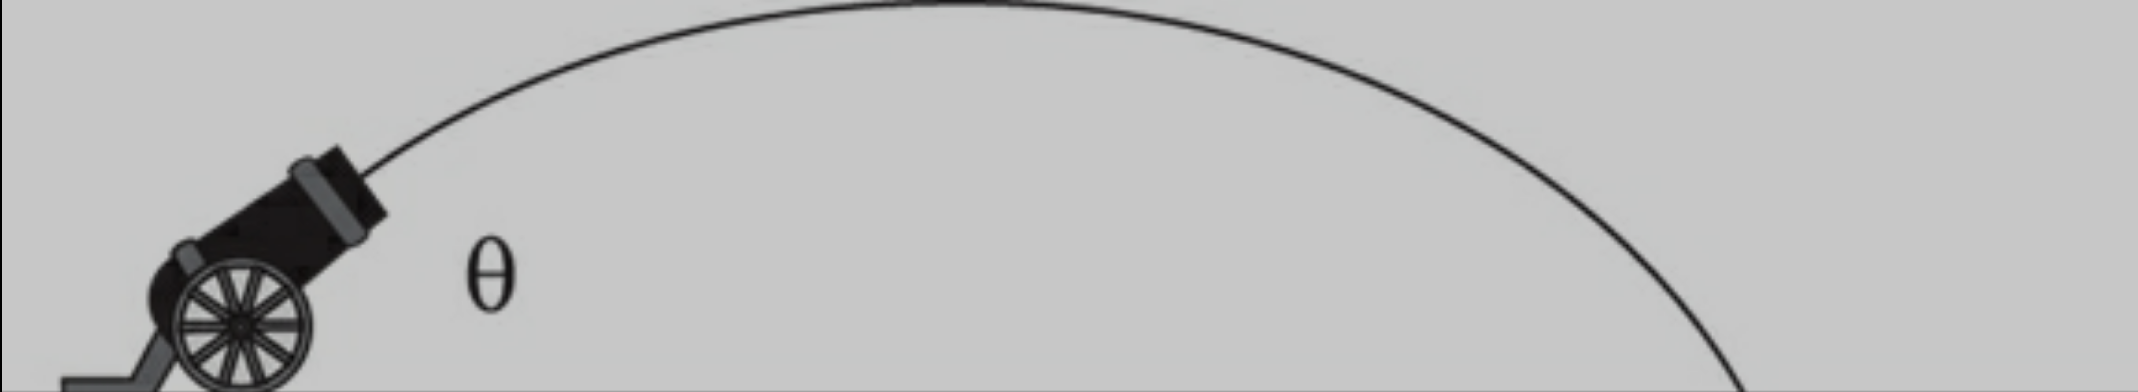
\includegraphics[width=\columnwidth]{image}
\\\\
Holzner, Steven. Physics I For Dummies (For Dummies (Math \& Science)) (p. 116). Wiley. Kindle Edition.
\\\\
\section{Solution}
The question we have to
\[ a=\frac{\triangle{v}}{\triangle{t}} \]
\[ -9.8=\frac{0-860\sin(45)}{t} \]
This is the time it takes to reach the apex. It would then have to travel back down.
\[ t = 62*2 = 124s \]
\[ s=\bar{v}t \]
The cannonball wouldn't magically stop after hitting the ground so we would assume it's final velocity doesn't change.
\[ \bar{v} = \frac{v_i+v_f}{2} \]
\[ \bar{v} = \frac{860 + 860}{2} = 860 \]
\[ s=\bar{v}t \]
\[ 860*\cos(45)*124 \]
\[ s=75,405m \]
\end{document}
